\clearpage
\subsubsection{MSVC + \olly}
\myindex{\olly}

2 pairs of 32-bit words are marked by red in the stack. 
Each pair is a double-number in IEEE 754 format and is passed from \main.

We see how the first \FLD loads a value ($1.2$) from the stack and puts it into \ST{0}:

\begin{figure}[H]
\centering
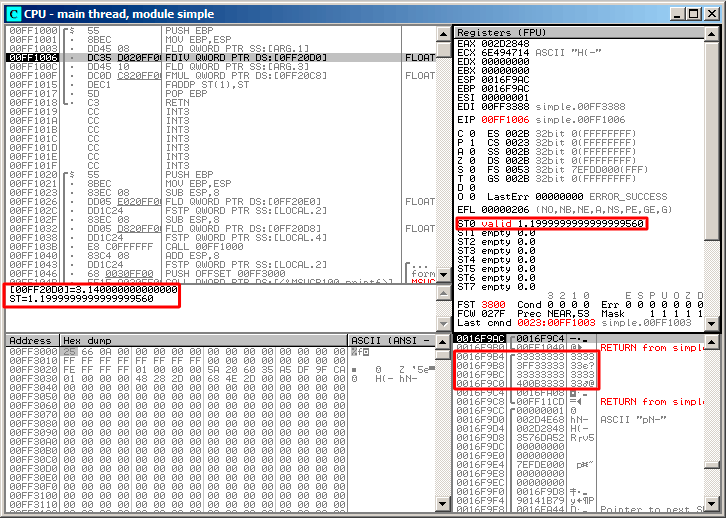
\includegraphics[scale=\FigScale]{patterns/12_FPU/1_simple/olly1.png}
\caption{\olly: first \FLD executed}
\label{fig:FPU_simple_olly_1}
\end{figure}

Because of unavoidable conversion errors from 64-bit IEEE 754 floating point to 80-bit
(used internally in the FPU), here we see 1.999\ldots, which is close to 1.2.

\EIP now points to the next instruction (\FDIV), which loads a double-number (a constant) from memory.
For convenience, \olly shows its value: 3.14

\clearpage
Let's trace further. 
\FDIV was executed, now \ST{0} contains 0.382\ldots
(\gls{quotient}):

\begin{figure}[H]
\centering
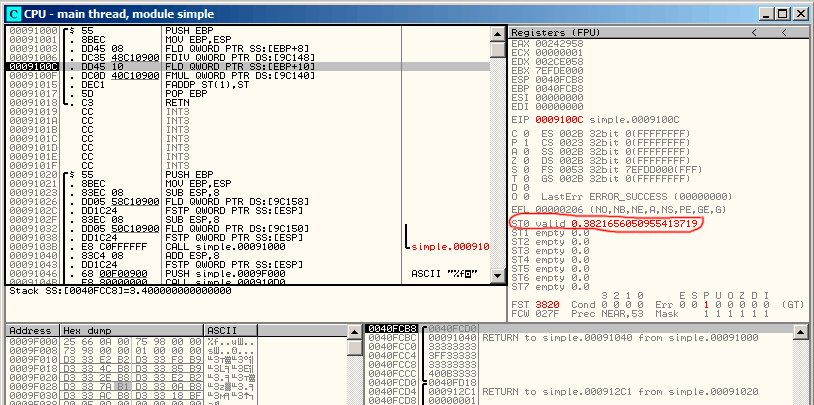
\includegraphics[scale=\FigScale]{patterns/12_FPU/1_simple/olly2.png}
\caption{\olly: \FDIV executed}
\label{fig:FPU_simple_olly_2}
\end{figure}

\clearpage
Third step: the next \FLD 

was executed, loading 3.4 into \ST{0} (here we see the approximate value 3.39999\ldots): 

\begin{figure}[H]
\centering
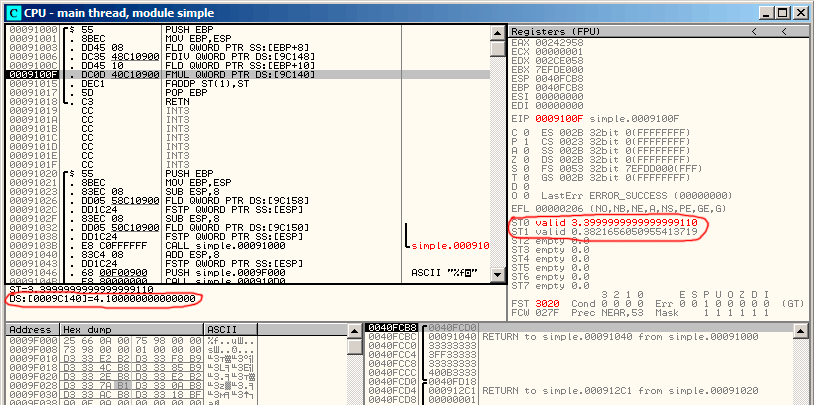
\includegraphics[scale=\FigScale]{patterns/12_FPU/1_simple/olly3.png}
\caption{\olly: second \FLD executed}
\label{fig:FPU_simple_olly_3}
\end{figure}

At the same time, \gls{quotient} \IT{is pushed} into \ST{1}.
Right now, \EIP points to the next instruction: \FMUL. 
It loads the constant 4.1 from memory, which \olly shows.

\clearpage
Next: \FMUL %
was executed, so now the \gls{product} is in \ST{0}:

\begin{figure}[H]
\centering
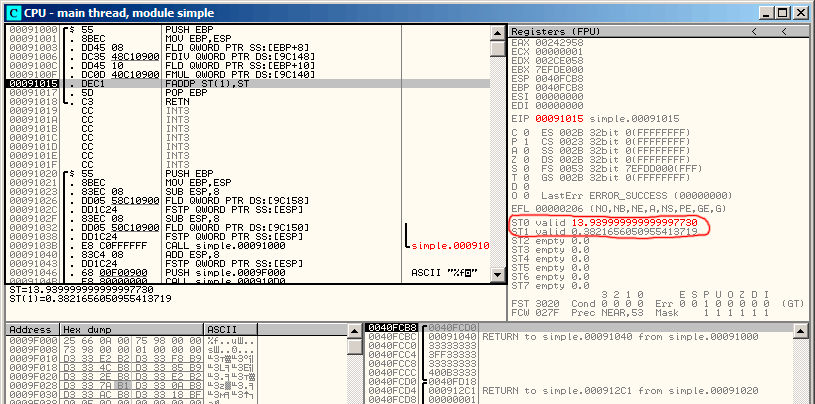
\includegraphics[scale=\FigScale]{patterns/12_FPU/1_simple/olly4.png}
\caption{\olly: \FMUL executed}
\label{fig:FPU_simple_olly_4}
\end{figure}

\clearpage
Next: \FADDP was executed, now the result of the addition is in \ST{0}, and \ST{1} is cleared:

\begin{figure}[H]
\centering
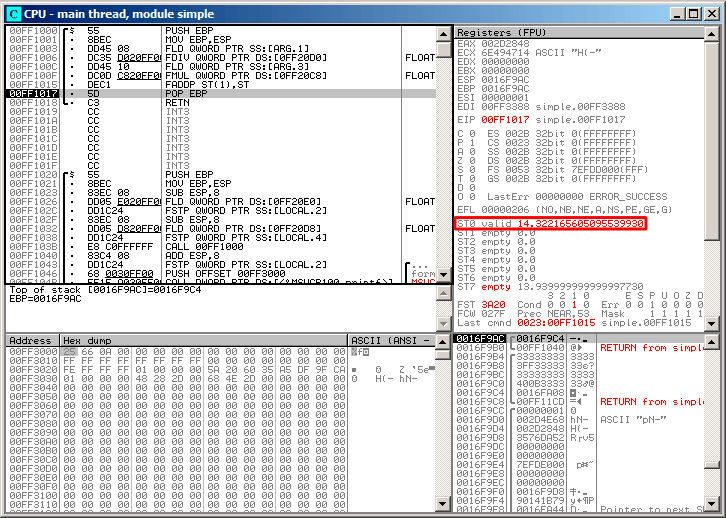
\includegraphics[scale=\FigScale]{patterns/12_FPU/1_simple/olly5.png}
\caption{\olly: \FADDP executed}
\label{fig:FPU_simple_olly_5}
\end{figure}

The result is left in \ST{0}, because the function returns its value in \ST{0}.

\main takes this value from the register later.

We also see something unusual: the 13.93\ldots value is now located in \ST{7}.
Why?

\label{FPU_is_rather_circular_buffer}

As we have read some time before in this book, the \ac{FPU} registers are a stack: \myref{FPU_is_stack}. 
But this is a simplification.

Imagine if it was implemented \IT{in hardware} as it's described, then all 7 register's
contents must be moved (or copied) to adjacent registers during pushing and popping, 
and that's a lot of work.

In reality, the \ac{FPU} has just 8 registers and a pointer (called \GTT{TOP}) which contains a register number,
which is the current \q{top of stack}.

When a value is pushed to the stack, \GTT{TOP} is pointed to the next available register,
and then a value is written to that register.

The procedure is reversed if a value is popped, however, the register which was freed is not cleared
(it could possibly be cleared, but this is more work which can degrade performance).
So that's what we see here. 

It can be said that \FADDP saved the sum in the stack, and then popped one element.

But in fact, this instruction saved the sum and then shifted \GTT{TOP}.

More precisely, the registers of the \ac{FPU} are a circular buffer.
